% \documentclass[draft,final]{vutinfth} % Remove option 'final' to obtain debug information.
\documentclass[draft, final]{vutinfth} % Remove option 'final' to obtain debug information.

% Extended LaTeX functionality is enables by including packages with \usepackage{...}.

\usepackage{amsmath}    % Extended typesetting of mathematical expression.
\usepackage{amssymb}    % Provides a multitude of mathematical symbols.
\usepackage{mathtools}  % Further extensions of mathematical typesetting.
\usepackage{microtype}  % Small-scale typographic enhancements.
\usepackage[inline]{enumitem} % User control over the layout of lists (itemize, enumerate, description).
\usepackage{multirow}   % Allows table elements to span several rows.
\usepackage{booktabs}   % Improves the typesettings of tables.
\usepackage{subcaption} % Allows the use of subfigures and enables their referencing.
\usepackage[ruled,linesnumbered,algochapter]{algorithm2e} % Enables the writing of pseudo code.
\usepackage[dvipsnames,table]{xcolor} % Allows the definition and use of colors. This package has to be included before tikz.
\usepackage{nag}       % Issues warnings when best practices in writing LaTeX documents are violated.
\usepackage{todonotes} % Provides tooltip-like todo notes.
\usepackage{fontspec} % Determines font encoding of the output. Font packages have to be included before this line.
\usepackage{hyperref}  % Enables cross linking in the electronic document version. This package has to be included second to last.
\usepackage[acronym,toc]{glossaries} % Enables the generation of glossaries and lists fo acronyms. This package has to be included last.

\uselanguage{english}
\bibstyle{plain}
\bibdata{main}
% \setmainfont{Source Serif 4}
% \setsansfont{Source Sans 3}
% \setmonofont{Fira Code}
% Define convenience functions to use the author name and the thesis title in the PDF document properties.
\newcommand{\authorname}{Daniel Jonas Otto} % The author name without titles.
\newcommand{\thesistitle}{Virtual Reality as a Catalyst for the Energy Transition} % The title of the thesis. The English version should be used, if it exists.

% Set PDF document properties
\hypersetup{
    pdfpagelayout   = TwoPageRight,           % How the document is shown in PDF viewers (optional).
    linkbordercolor = {Blue},                 % The color of the borders of boxes around crosslinks (optional).
    pdfauthor       = {\authorname},          % The author's name in the document properties (optional).
    pdftitle        = {\thesistitle},         % The document's title in the document properties (optional).
    pdfsubject      = {Subject},              % The document's subject in the document properties (optional).
    pdfkeywords     = {a, list, of, keywords} % The document's keywords in the document properties (optional).
}

\setpnumwidth{2.5em}        % Avoid overfull hboxes in the table of contents (see memoir manual).
\setsecnumdepth{subsection} % Enumerate subsections.
\nonzeroparskip             % Create space between paragraphs (optional).
\setlength{\parindent}{0pt} % Remove paragraph identation (optional).
\newgeometry{top=2.5cm, bottom=2.5cm}
\OnehalfSpacing
% \sloppy
\hyphenpenalty=800
\tolerance=2000
\emergencystretch=3em

\makeindex      % Use an optional index.
% \makeglossaries % Use an optional glossary.
%\glstocfalse   % Remove the glossaries from the table of contents.

% Set persons with 4 arguments:
%  {title before name}{name}{title after name}{gender}
%  where both titles are optional (i.e. can be given as empty brackets {}).
\setauthor{}{\authorname}{}{male}
\setadvisor{Dipl.-Ing.in Dr.in}{Katharina Krösl}{}{female}

% For bachelor and master theses:
% \setfirstassistant{Pretitle}{Forename Surname}{Posttitle}{male}
% \setsecondassistant{Pretitle}{Forename Surname}{Posttitle}{male}
% \setthirdassistant{Pretitle}{Forename Surname}{Posttitle}{male}

\setregnumber{11811332}
\setdate{11}{1}{2024} % Set date with 3 arguments: {day}{month}{year}.
\settitle{\thesistitle}{Virtual Reality as a Catalyst for the Energy Transition}
% \setsubtitle{Optional Subtitle of the Thesis}{Eine wissenschaftliche Untersuchung des Potenzials von VR-Technologien in der Umweltbildung und -kommunikation}
\setthesis{bachelor}
\setcurriculum{Software and Information Engineering}{Software und Information Engineering}


\begin{document}
\frontmatter
\addtitlepage{ngerman}
\addstatementpage

\begin{acknowledgements*}
  Thank you to everyone who supported me in the creation of this work. I would especially like to thank my partner Astrid Gaderbauer for her support and understanding throughout the duration of this work. I would also like to thank Helwin Prohaska for his valuable advice and support in the development of the VR application. Additionally, I would like to thank my grandparents for their financial support and encouragement. Finally, I would like to thank my supervisor Katharina Krösl for her guidance and feedback throughout the entire work.
\end{acknowledgements*}

% \begin{kurzfassung}
% \todo{Ihr Text hier.}
% \the\baselineskip
% % print fontsize
% \the\fontdimen6\font
% \end{kurzfassung}

\begin{abstract}
This thesis presents the development of a Virtual Reality (VR) application aimed at facilitating the energy transition in Austria. It addresses the widespread perception of the energy transition as overly complex and unachievable, a view that has often led to political inaction and public uncertainty. Through the use of VR technology, this research seeks to demonstrate the necessity and feasibility of transitioning towards renewable energy sources, countering the prevailing skepticism and inertia.

The core of this study lies in creating an immersive VR experience that elucidates the concepts and advantages of the energy transition in an engaging and understandable manner. The application is designed to simplify complex environmental principles, making them accessible and relatable to users. By doing so, it aims to inspire a sense of urgency and possibility regarding the adoption of sustainable energy practices.

This work is grounded in the belief that technological innovation, particularly in the realm of VR, can play a crucial role in environmental advocacy. The goal is to empower individuals with knowledge and perspective, contributing to a more proactive and optimistic approach to environmental challenges in Austria.

The findings and developments from this thesis are expected to offer new pathways in environmental education and communication, highlighting how VR can be a potent tool in promoting understanding and action in the face of environmental challenges. This research aims to stand as a testament to the power of technology in driving societal change, especially in contexts where political leadership may be lacking.
\end{abstract}

\tableofcontents % Starred version, i.e., \tableofcontents*, removes the self-entry.
\mainmatter

\chapter{Introduction}

% One sentence or short paragraph about what the paper is about and a mini-summary of your main results. (1 par) 


% Introducing the important problem you solve, give some (possibly simplified) definitions (1 par)


% Why is this problem important, who has attempted to solve it, which solutions exist so far, why aren‘t they sufficient, why are we left with a dilemma, what are the main obstacles, why would it be useful to fight them. What would be the benefit of a (better) solution. (1/2 page)

...

research questions:
%Wie können die Möglichkeiten von VR genutzt werden, um grundlegendes Verständnis für die Energiewende zu schaffen und die Funktionsweise eines erneuerbaren Energiesystems zu vermitteln?
%1) nutzen von VR generell für verständnis /akzeptanz
1) Can a VR simulation such as the VR application of Energiewende Linz (Kaisergasse VR?) increase understanding/acceptance  and interest for climate-friendly technologies? 

%2) vorteil einer interaktiven sim für photovoltaic
2) Can an interactive photovoltaic use case increase understanding and acceptance of PV solutions?


% Elaboration on single obstacles and how you overcome them.



% Short description of results and their advantage and usefulness in chronological order.


% Some remarks about the nontriviality of the solution 



% Summary of main results in form of a dotlist

contribution:
-) user study and evaluation of Kaisergasse VR
-) use case designed and implemented (derive from related work) ... as educational tool?
-) user study to evaluate the benefit of a more interactive solution


% Further related work and a sentence about future plans




% Roadmap „This paper is organized as follows... 




This bachelor thesis is dedicated to the development of an innovative Virtual Reality application, which aims to advance the energy transition in Austria. In a context where public opinion and media coverage in Austria often show a certain skepticism towards the energy transition and its challenges, this work aims to bring a positive change and deeper understanding through the use of VR technology.

In Austria, the energy transition is often perceived as complex and controversial in public debate and the news. There is an urgent need to communicate more clearly the benefits and feasibility of this transition. This bachelor thesis aims to positively influence public opinion and promote a deeper understanding of its importance by creating a VR application that conveys the principles and benefits of the energy transition in an interactive and immersive manner.

The work intends to explore the role of VR as a powerful tool in education and communication strategies, to create broader awareness and stronger support for the energy transition among the Austrian population. In doing this, I utilize the latest developments in VR technology and combine them with current environmental issues.

My goal is to make a scientifically founded contribution that considers both the technological aspects and the didactic principles in conveying the challenges and solutions of the energy transition. The work is intended to serve as a basis for future research and applications dealing with the use of VR technology in environmental education and communication.






\chapter{Related Work}

% am besten du machst dir hier als erstes mal ein paar stichworte zur struktur und den main take-aways
% sowas wie:
% VR wird viel in education verwendet (in unterschiedlichen gebieten
% dabei ist besonders wichtig/beneficial/etc: 
% orientierung 
% interaktivität
% collaboration
% ...
% das hab ich jetzt so bissl aus deinem related work raus gelesen. das sind aber eigentlich dinge die gut sind für die argumentation/motivation und daher in die introduction passen. im related work geht es eher darum den state of the art in dem bereich zusammenzufassen. also was gibt es für ähnliche arbeiten? wie unterscheiden sich die? wie sind die besser oder schlechter, etc.

\section{Virtual Reality in Education}

A central aspect in the discussion about the use of Virtual Reality (VR) in education is addressed by Radić-Weissenfeld et al.\cite{hu2017virtual}. This paper offers a profound insight into the diverse applications and the potential of VR as an educational tool in today's era of experience and interactivity.

The authors discuss how VR technologies can revolutionize learning by creating immersive and interactive environments that enable learners to experience complex concepts and systems in a way that is not possible with traditional teaching methods. This approach, aimed at making abstract theories tangible through direct experience, is particularly relevant for the fundamental understanding of the energy transition and renewable energy technologies. The authors emphasize that VR technology offers the possibility to enable learners to experience the impacts of their decisions and actions in a realistic environment. This approach is especially relevant for the energy transition, as it allows learners to understand and experience the effects of their decisions on the environment.

In the context of my work, which aims to improve understanding of the functioning of renewable energy systems through VR, this article provides important insights. The principles of immersion and interactivity described in the article are fundamental pillars for the development of the VR application. In particular, the emphasis on "experience orientation" in the learning process is important for the project, as it is about giving users a deep understanding of the dynamics and impacts of various photovoltaic configurations.

Radić-Weissenfeld et al. also underline the importance of user-centricity in VR learning environments. This aspect is crucial to ensure that our VR application is not only informative but also user-friendly and engaging. By applying these principles, we can create a learning experience that is not only educational but also motivating and inspiring for users.

In conclusion, the article by Radić-Weissenfeld et al. provides an important foundation for our project by demonstrating how VR technology can be effectively used in educational contexts. The insights gained from this directly flow into the design of our VR application, with the goal of creating an intuitive and effective learning experience around the topic of energy transition.
% welche erkenntnisse konkret?

\section{VR Technology in Higher Education: New Perspectives and Applications}

Virtual Reality has established itself as a powerful tool in higher education, especially in the STEM fields (Science, Technology, Engineering, and Mathematics), where VR is predominantly used to make complex and abstract concepts more comprehensible~\cite{ding2022review}. The immersive properties of VR enable students to not only theoretically learn technical and scientific processes but also to grasp them practically and visually, leading to a deeper understanding. This application of VR highlights the technology's potential to make challenging topics more accessible and tangible.

Ding and Li ~\cite{ding2022review} ran a study with ... students to investigate... Their results showed that VR has a significant impact on students' learning outcomes. The use of VR technology in higher education has been observed to improve the absorption and retention of knowledge. VR offers a unique, interactive learning experience that complements and surpasses traditional teaching methods by immersing students directly in the learning environment. This direct, experience-based learning method not only fosters an understanding of complex scientific and technical concepts but also improves long-term retention.

Furthermore, the study emphasizes that VR positively influences students' learning behavior. The incorporation of VR into curricula leads to increased engagement and motivation among students. This technology allows learners to experiment and explore in an interactive and dynamic environment, making learning an active and captivating experience. This not only arouses interest in the subject matter but also enhances problem-solving and critical analysis skills. These changes in student behavior contribute to increasing learning success and fostering a deeper, lasting interest in the topics.

\section{Significant Developments in Educational Virtual Environments}

Mikropoulos and Natsis~\cite{mikropoulos2011educational} provide a comprehensive analysis of research in the field of education-oriented virtual environments (VE) over a ten-year period. This extensive review illuminates the crucial developments and changes that virtual educational environments have undergone in the last decade, thus providing an indispensable basis for understanding the current and future trends in this field.

Mikropoulos and Natsis focus on the diverse applications of VEs in education. They note that VEs are increasingly recognized as effective tools that enrich learning through their immersive and interactive properties in different application areas, from scientific subjects to complex social and cultural topics.

They argue that interactive elements in virtual educational environments can increase learner engagement and motivation, leading to a deeper and more sustainable understanding of the learning content.

Moreover, the authors emphasize the role of VEs in promoting collaborative learning. They demonstrate how virtual environments can support cooperative and collaborative learning, where students can jointly solve tasks and share knowledge, leading to improved understanding and higher retention. This approach is particularly effective as it emphasizes the social aspects of learning, which are often neglected in traditional learning environments.

The researchers also point out the challenges associated with implementing VEs in educational institutions. These challenges include technical limitations, high costs for setting up and maintaining such systems, and the need for adequate training for teachers to effectively use these technologies. They stress the importance of careful planning and support from educational institutions to overcome these challenges.

In conclusion, Mikropoulos and Natsis underscore the potential of VEs as transformative tools in education. They argue that these technologies, when effectively utilized, can revolutionize learning and lead to deeper, more meaningful educational experiences. Their research suggests that VEs could play a key role in shaping future educational strategies, especially in areas that require a high degree of interactivity and engagement.

Given these insights, it is clear that the work of Mikropoulos and Natsis makes an important contribution to the understanding and further development of virtual educational environments. Their research findings provide valuable insights for educational professionals, developers, and researchers working at the intersection of technology and education, forming a solid foundation for future exploration and implementation of VEs in educational contexts.

The insights of Mikropoulos and Natsis are of central importance to my project. Their paper not only offers a deep insight into the historical development and various application areas of virtual educational environments but also serves as a valuable source of inspiration for innovative teaching methods in virtual reality. The importance they place on interactivity in virtual environments is particularly relevant to my project. They provide concrete starting points for designing an interactive and engaging VR learning environment, aiming not just to entertain users but actively involve them in the learning process.

Furthermore, understanding the challenges discussed by Mikropoulos and Natsis -- particularly regarding technical, financial, and pedagogical aspects -- opens the possibility to plan and implement my project realistically and purposefully. This will be crucial for ensuring smooth integration and acceptance of the VR learning application in educational contexts.

In conclusion, the paper forms a sound basis for the development of my VR application. It serves as a compass that highlights both the potentials and pitfalls of using Virtual Reality in education. By taking these insights into account, I can develop an application that is not only technologically advanced but also pedagogically valuable, thus creating an effective and appealing learning experience for users.

\section{Effectiveness and Integration of VR-based Instruction}

The integration of VR-based instruction into traditional teaching methods is a central element of my literature review. This topic is extensively analyzed in the paper "Effectiveness of virtual reality-based instruction on students' learning outcomes in K-12 and higher education"\cite{merchant2014effectiveness}. This meta-analysis explores the effectiveness of VR in various educational contexts and details the specific conditions under which VR can significantly influence learning success. Therefore, it provides valuable insights for the effective use of VR in educational environments. The results are particularly relevant for our project due to the matching age group of the participants and the thematic focus on declarative learning objectives.

Key findings of the paper are:
\begin{itemize}
  \item The results show that VR-based educational environments significantly improve students' learning outcomes. This underscores the potential of VR as an effective tool in education.

  \item The type of learning outcomes, whether knowledge or skill acquisition, influences the effectiveness of VR-based instruction. VR is particularly effective in imparting declarative knowledge. This is relevant for our project as we focus on conveying knowledge about the functioning of photovoltaic systems and the effects of various configurations.

  \item A combination of VR and other teaching methods proves to be particularly effective. This supports an integrated teaching approach where VR is used as a complement to traditional teaching forms. This approach is particularly relevant for our project as we develop the VR application as an addition to workshops in schools.

  \item The nature of feedback and the type of learning tasks are crucial for the effectiveness of VR in an educational context. Detailed explanations are more effective for declarative tasks, while concrete feedback on the correct answer is more effective for procedural tasks. This underlines the importance of tailoring feedback to the type of learning task.

  \item The methodological rigor of study designs influences the observed learning outcomes, with higher methodological rigor leading to stronger evidence of VR's effectiveness. This highlights the importance of careful design of VR-based educational environments.

  \item The results show that VR environments in education increase learner engagement and motivation. Thus, VR serves as a tool to arouse students' interest and actively involve them in the learning process.
\end{itemize}

This paper provides valuable insights for the effective design of VR-based educational environments for my work. It emphasizes the need to carefully design VR applications to ensure they support and complement learning objectives. The insight that a combination of VR and other teaching methods, as well as tailoring feedback to the type of learning task, is crucial for the success of VR in education. These insights will be considered in developing our VR application to ensure an optimal and effective learning experience.

The effectiveness of combining VR with traditional teaching methods highlighted in this paper is already being applied in our project. Our VR application is used in school workshops to make the more abstract content tangible and comprehensible, complementing frontal teaching. This methodological connection helps regain the attention of young people and deepens their understanding of the complex topics of the energy transition. Notably, the potential influence on knowledge retention is enhanced by the interactive and immersive nature of VR.

Based on the findings from the mentioned paper and previous research, I can further develop the VR application by integrating the following elements:

\begin{itemize}
  \item Implementation of interactive feedback systems that allow learners to receive immediate and specific feedback on their actions and decisions within the VR environment. This can be realized, for example, through real-time simulation data and explanatory notes.

  \item Integration of appealing and informative data visualizations that enable users to visualize the immediate effects of their decisions on the environment and energy efficiency. Such visualizations could dynamically display changes in energy amounts, CO2 emissions, or costs depending on the chosen parameters.

  \item Development of additional interactive modules that address specific aspects of the energy transition. These could include simulations that illustrate the effects of different energy systems under selected environmental conditions.

  \item By providing various interaction options within the VR environment, different learning styles can be accommodated. This can be enabled through options for exploratory and structured learning.

  \item Ensuring that the VR application is seamlessly integrated into the preceding and subsequent content of the workshops to create a coherent learning experience. This could be achieved by providing accompanying materials and by coordinating and preparing the content with the teachers.

\end{itemize}

Although the integration of VR into traditional teaching methods is promising, we should review and adjust the effectiveness and relevance of the VR application as necessary. It is important to gather feedback from teachers and students and optimize the application accordingly to ensure that it meets learning objectives and effectively contributes to knowledge transfer.

The insights from the paper and previous studies support the further development of the VR application as an effective tool in education for the energy transition. By specifically adapting and expanding the application, we can further increase learning success and foster lasting interest in the topic. Future research and applications could focus on optimizing the interaction between VR and traditional teaching methods and examining the effects on different learning groups.


\section{VR Applications for Renewable Energy}
% related work
% Works focusing on the use of VR in environmental education and awareness.
% what, how, result, relevance


\chapter{Approach}

The association \href{https://www.energiewende-linz.at}{Energiewende Linz} presented their first exhibition at the Ars Electronica Festival in 2022 under the name "PowerPlayGround". This exposition aimed to present multiple interactive stations, each delving into a different aspect of the climate crisis and energy transition. The centerpiece of the exhibit was the recently completed \href{https://www.pilotprojekt-kaisergasse.at/}{Pilotprojekt Kaisergasse Phase 1}, which outlined a comprehensive strategy for making the residential building Kaisergasse 20 Linz more climate-friendly. To visually demonstrate the proposed solutions, the "Kaisergasse VR" Virtual Reality application was developed, effectively building on the thematic groundwork established by the preceding stations and strengthening understanding of the solutions.

Participants in "Kaisergasse VR" begin their journey in the courtyard of Kaisergasse 20, where they can use a watering can to change dusty dirt into a lush, wild meadow with some trees, visually reducing the surrounding temperature as indicated by a thermometer. The addition of greenery to two nearby commercial building rooftops brings the temperature down to a comfortable 24°C. Accessing these rooftops involves the use of flight capabilities, which are facilitated by the controllers for ascending or descending, with gravity turned off for easy navigation. On the roof of the residential building, semi-transparent solar panel templates became visible. Interacting with these templates via the controllers causes the installation of panel groups, which tints the cables green to indicate electricity generation.
Interacting with these templates via the controllers triggers the installation of panel groups, which turns the cables green to represent electricity generation. Exploring further to the courtyard's garages and parking spots shows four plugs that have been activated by the photovoltaic system. Engaging with these connectors enables the construction of cables to electric car charging stations, visibly discerning which cars are being charged.
Throughout the virtual environment, numerous bubbles invite interaction; clicking on these bubbles reveals 360° photographs that provide a panoramic glimpse into reality, enhancing the experience by bridging the gap between virtual and real-world visuals.

\section{Photovoltaic Simulation}
the next section is about explaining how my bachelor thesis project directly builds upon this groundwork. Helwin approached me  if i want to team up. By building the next evolution of the initial app (more like a mvp) i am able to help bringing the energiewende a step further. My application would  be used at ars electronica and workshops he is holding. this should enable us to improve understanding and engagement of many people for climate friendly technologies and actions. 

After some brainstorming it was clear that focusing on one aspect and do it well would wield the best results and are perfect workpiece for my bachelor thesis. Educatiion around the functionality and advantages of photovoltaic systems seemed a very promising endeavor. It is also the aspect where the existing application lacked the most, in my personal opinion.

%I was very excited about helping in making austria more future proof and climate friendly. Developing games was my childhood dream, quite forgotten and labeled unrealistic, this was my big chance in pursuing something meaningful for the future and myself. To build upon the existing application and reuse whats already built, i decided to learn unreal engine from scratch, instead of considering to alternative VR-friendly options like unity and godot. In hindsight it may seem overkill but i completely worked through the tutorials by UnrealSensei and then GameDevTV. This also incorporated in depth the programming of game functionality in C++. This learning stage was extensive and spanned over 4 months.

Subsequently my plan was to use the whole summer to complete the application is best possible condition for the Ars Electronica 2023. Helwin additionally hired the original Developer to fix several bugs in the application and improve the disappointing performance. Working as multiple Developers on the same game is very challenging in Unreal Engine as in any other engine. The game files are binary and impossible to merge different changes through git. To make matters worse the other developer refused to communicate or cooperate. I ended up reapplying my changes over and over when merging the main branch into my new feature. Additionally i volunteered to help realize 2 additional new games which would be showcased in the exhibition. One featured a highly realistic forest fire, the second featured a flood scenario where you are tasked to save the village from the water masses by building dams. I worked around the clock every day to also finish my own application in time. But sadly It just was impossible, regarding my lack of experience and worn mental state.

The Exhibition went smoothly, despite of numerous hardware faults. Following that i had to fully focus on my family and me moving to a new apartment. I was heavily exhausted and was not able to tackle writing the chapter 

%describe the concept:
%1) the whole VR project of Energiewende Linz
%2) new use case (more focus here)

\chapter{Implementation}

implementation details
describe the technology (UE, plugins)
structure
interesting difficult detail (feedback loop)

\chapter{Evaluation}
\section{Baseline User study}
The first user study aimed at creating a baseline, which was important for both the academic standard and the project's viability. It involved analyzing the original application to find its fundamentals. Rather than inventing the wheel, this was about refining it and removing any major defects to demonstrate empirically that VR can, in fact, be a catalyst for increasing awareness of, interest in, and support for climate-positive projects. The main focus of our research was a survey intended to assess the original application's usefulness and provide direction for its successor. We were able to provide a clear picture of our participants' baseline knowledge, attitudes, and potential effects of VR on climate action because of this comprehensive approach.

Recruitment was opportunistic, utilizing the "JKU Games 2023S" event to engage with a diverse group of attendees. We invited all interested individuals to enter our virtual reality experience, with no particular selection criteria. Despite its scope, this method offered a useful variety of user experiences and input. Every participant received guidance throughout the virtual reality experience to make sure they could easily navigate the application's features. After being taken to the courtyard inside the application, participants were able to take part in a range of climate-friendly activities. A disappointing user experience was caused by a combination of flight mechanics and poor frame rates, highlighting the crucial role of technical proficiency in the development of VR applications. Participants were subsequently asked to complete our online survey about their experience.

The event JKU Games 2023S attracted young visitors who were interested in gaming and open to trying virtual reality. Given their familiarity with digital environments and interactive experiences, these participants brought a unique perspective to the evaluation, potentially setting higher standards for interactivity and immersion.

    %how many participants (demographics), user study protocol (list)
    
\section{Final study}
The VR-Day event was hosted at HLW Steyr, organized by Lea and Fabio as part of their diploma project on digitalization. Initially planned for two classes, the event was attended by one due to a rescheduling caused by my illness. The morning was dedicated to a 2-hour technical setup, which went smoothly except for an issue with one Quest 2 controller. At 11 AM, we loaded the equipment and headed to the venue. The workshop spanned three hours, from 1 PM to 4 PM.

Helwin kicked off with a presentation about the Energiewende Linz association, highlighting the challenges of the energy transition and previous projects, including exhibitions at Ars Electronica 2023. Subsequently, approximately 20 students had the opportunity to experience VR games like Richie's Plank and Beat Saber on two PC-VR stations equipped with Meta Quest 2, and one with Quest 2. Two additional PC-VR stations featured a Quest 2 and a Quest 3, showcasing the photovoltaic simulation I developed. Initially, there was a noticeable lack of interest among the students in trying the simulation, but through some persuasion, I managed to engage a few participants for the study. The feedback received was overwhelmingly positive.

The procedure for the simulation demonstration was as follows: I approached individuals directly, inquiring if they were interested in trying the simulation and participating in the user study. After explaining the controls and interaction possibilities through a presentation, participants were free to explore the simulation at their leisure. Upon completion, they were asked to complete a feedback form via a QR code link on their mobile devices. While I did not track the completion rate, I received 10 filled forms, including those from Lea and Fabio.

We encountered several technical issues with the VR headsets throughout the day: one displayed a recurring black screen, another had involuntary forward motion (noted during the morning setup), and another faced connection issues with the PC. Additionally, a borrowed laptop froze during a Beat Saber session.

Seeking more feedback, Helwin later facilitated a session with 6 individuals at HTL Linz, where 5 completed the questionnaire.

Furthermore, I presented the simulation to my colleagues at work on March 4, 2023. The 6 participants liked the experience and i was able to get 3 filled surveys.

\chapter{Results}
\section{Understanding the Impact of "Kaisergasse VR" on Climate-Friendly Technologies}
The "Kaisergasse VR" simulation aimed to bring the real-world project of installing photovoltaic panels on residential housing to a wider audience. To share the project's experiences, a VR visualization was created for an exhibition at Ars Electronica, assuming that the background information would be provided in a preceding lecture. As a result, the VR functionality was designed to be straightforward.

In the "Kaisergasse VR" experience, users can engage in a few key activities: installing groups of PV panels with a few clicks, drawing cables from the house to the charging stations to power them for electric vehicles, and using a "brush" to greenify the courtyard and surrounding flat roofs, which in turn reduces the ambient temperature. The intention behind allowing users to implement these measures themselves within the VR environment is to help them understand and potentially support or initiate similar actions in their own surroundings.

To evaluate the impact of the "Kaisergasse VR" on participants' understanding, the responses to the questions will be analyzed statistically. The mean ratings for each question will be calculated to ascertain the overall effectiveness of the VR experience in conveying the intended information. The results will shed light on the potential of VR as an educational tool in promoting sustainable practices and technologies.

\section{Can a VR simulation such as the VR application of Energiewende Linz ("Kaisergasse VR") increase understanding of and interest in climate-friendly technologies?}
Statistical tests will be conducted to compare the mean scores from the preliminary and final study, allowing for the assessment of any significant changes in participants' understanding post-interaction with the VR simulation.

\textbf{Hypothesis 1:} VR applications such as "Kaisergasse VR" enhance participants' understanding of climate-friendly technologies.

We'll analyze participant responses to post-experience questions aimed at assessing their understanding. The questions, rated on a 1 to 5 scale (with 5 indicating a high level of understanding and 1 indicating a low level), include:
\begin{itemize}
    \item Did the VR experience help you understand the actions that can be taken to improve urban thermal conditions?
    \item Did the VR experience help you understand the benefits of these actions?
\end{itemize}
We anticipated that scores above the midpoint of 3 would indicate a successful enhancement in understanding due to the VR experience.

\begin{figure}[h]
  \centering
  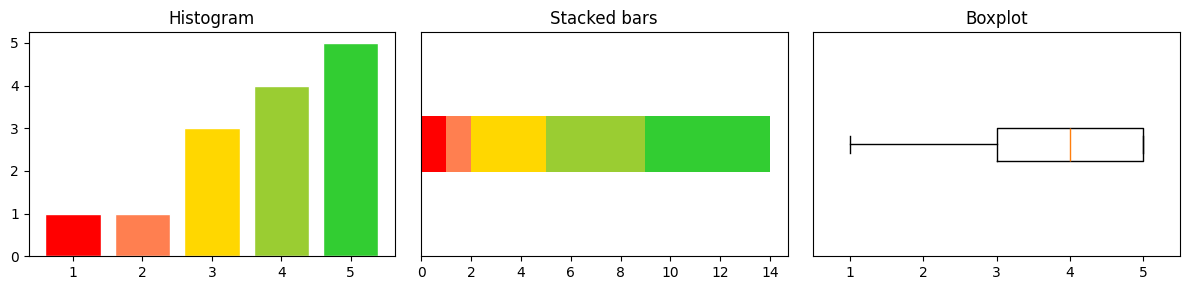
\includegraphics[width=\textwidth]{test1.png}
  \caption[Distribution of answers for question 1.1]{Distribution of answers for question 1.1}
  \label{fig:analysis-image}
\end{figure}

Initially, the Shapiro-Wilk test was applied to check for normality in the response distribution, yielding values of 0.865 (p=0.036) and 0.874 (p=0.048) for the two questions, respectively. These results indicated a deviation from normal distribution, necessitating the use of the non-parametric Wilcoxon test suited for small, non-normally distributed samples.

The Wilcoxon test produced a statistic of 54.5 with a p-value of 0.02466 for the first question and a statistic of 45.0 with a p-value of 0.03301 for the second. These initial p-values suggested a statistically significant impact of the VR experience on understanding. However, after applying the Bonferroni correction to account for multiple comparisons, these findings were adjusted to be statistically insignificant, leading to the retention of the null hypothesis for both questions.

In conclusion, while the initial analysis hinted at a potential impact of the "Kaisergasse VR" on enhancing participants' understanding of climate-friendly technologies, the application of the Bonferroni correction revealed that these effects did not meet the threshold for statistical significance. This indicates that, based on this strict statistical criterion, the VR simulation did not significantly improve participants' understanding as initially hypothesized. Further research, possibly with a larger sample size or different methodological approaches, is suggested to explore the educational potential of VR in environmental awareness.

% present the results

\textbf{Hypothesis 2:} VR applications such as "Kaisergasse VR" stimulate increased interest in adopting climate-friendly technologies.

Participant responses to post-experience questions will assess their interest in adopting climate-friendly actions. Responses are rated on a 1 to 5 scale, with 5 indicating high likelihood and 1 indicating low likelihood:
\begin{itemize}
\item Would you be more likely to install a green roof after testing the VR simulation?
\item Would you be more likely to install a PV system on your roof after testing the VR simulation?
\item If you were to purchase a new car, would it be an electric vehicle?
\end{itemize}
The mean scores for each scenario will be calculated and compared against the scale's midpoint (a score of 3) to determine the VR simulation's influence on participants' interest. Scores significantly exceeding the midpoint will indicate a heightened interest in climate-friendly technologies attributable to the VR experience, thus supporting Hypothesis 2.The analysis will focus on the distribution of scores to understand the VR simulation's impact on interest levels.

% present the results

\section{Can an interactive photovoltaic use case increase understanding of and interest in PV solutions?}

\textbf{Hypothesis 3:} Interactive engagement with a photovoltaic use case in the VR application significantly enhances both understanding and interest in PV solutions.

To evaluate this hypothesis, we will analyze responses to two pivotal questions included in both the preliminary and final study questionnaires, focusing on the VR experience's role in deepening understanding of PV systems. Responses were gathered on a 1 to 5 scale, with 5 denoting "very helpful" and 1 denoting "not helpful at all."
\begin{itemize}
    \item Did the VR experience help you understand how a photovoltaic system can be utilized?
    \item Did the VR experience help you understand the benefits of a photovoltaic system?
\end{itemize}
The mean scores for each question will be calculated and compared between the preliminary and final studies. A significant increase in the mean scores in the final study would indicate an enhanced understanding attributed to the interactive PV use case in the VR experience.

% present the results

\section{How does an interactive VR simulation enhance factual knowledge regarding the optimal orientation of photovoltaic panels?}

This research question focuses on the VR simulation's capacity to enhance factual knowledge related to the strategic placement of photovoltaic panels to optimize electricity production throughout different times of the year.

\textbf{Hypothesis 4:} The interactive PV use case in the VR simulation significantly gain factual knowledge regarding the optimal orientation of PV panels.

To assess this hypothesis, participants' responses to specific knowledge-based questions were analyzed post-interaction with the VR simulation. These questions aimed to evaluate the understanding of PV panel orientation for maximum electricity generation in June, December, and over the year. The correct answers were predetermined based on technical PV system optimization principles and are marked in Bold:
\begin{enumerate}
    \item In which orientation does a single panel generate the most electricity in June?
    
    (a) \textbf{Flat}, (b) Tilted towards the South, (c) East-West tilt
    \item In which orientation does a single panel generate the most electricity in December?
    
    (a) Flat, (b) \textbf{Tilted towards the South}, (c) East-West tilt
    \item In which orientation does a single panel generate the most electricity throughout the year?
    
    (a) Flat, (b) \textbf{Tilted towards the South}, (c) East-West tilt
\end{enumerate}
The percentage of participants selecting the correct option for each question is calculated and compared to what would be expected from a random distribution. Given three choices for each question, a random guess would have a one-third chance of being correct. 

A significantly higher percentage of correct responses in the post-VR experience indicates that participants' understanding exceeds what would be expected by chance, thereby supporting Hypothesis 4. Statistical significance can be assessed using a one-sample proportion test against the expected proportion of 1/3 for random guessing.

To further analyze the data, we will examine the distribution of responses to determine if the observed pattern of correct answers significantly deviates from a random distribution. This will involve using a chi-square goodness-of-fit test, where the null hypothesis is that the distribution of answers conforms to random guessing, and the alternative hypothesis is that it does not, indicating that the VR experience had a tangible impact on participants' understanding.

% present the results

\chapter{Discussion}
interpretation of results

\chapter{Conclusion and Future Work}

\backmatter

% Use an optional list of figures.
\listoffigures % Starred version, i.e., \listoffigures*, removes the toc entry.

% Use an optional list of tables.
% \cleardoublepage % Start list of tables on the next empty right hand page.
% \listoftables % Starred version, i.e., \listoftables*, removes the toc entry.

% Use an optional list of alogrithms.
% \listofalgorithms
% \addcontentsline{toc}{chapter}{List of Algorithms}

% Add an index.
\printindex

% Add a glossary.
\printglossaries

% Add a bibliography.
\bibliographystyle{alpha}
% \bibliographystyle{plain}
\bibliography{main}

\end{document}
